% Capítulo 2
\chapter{Conceitos e Definições}
\label{conceitos}

%%%%%%%%%%%%%%%%%%%%%%%%%%%%%%%%%%%%%%%%%%%%%%%%%%%%%%%%%%%
\section{\texorpdfstring{\MakeUppercase{Grafo}}{}}
\label{conceitos__grafo}

Um \emph{grafo} G é um par ordenado (V[G], E[G]) sendo V[G] um conjunto de \emph{vértices} e E[G] um conjunto de \emph{arestas}, onde cada aresta é associada a um par não ordenado de vértices de G através de uma \emph{função de incidência} $\psi_{G}$. Seja \emph{e} uma aresta e \emph{u} e \emph{v} vértices em G, tais que $\psi_{G}$(\emph{e}) = \{\emph{u}, \emph{v}\}, assim, pode-se dizer que \emph{e} é uma aresta que \emph{incide} sobre \emph{u} e \emph{v} e que \emph{u} e \emph{v} são as \emph{extremidades} de \emph{e}. Além disso, é dito que \emph{u} e \emph{v} são vizinhos entre si.~\cite{bondy1976graph}.

O número de vértices e arestas em G são denotados por |V[G]| e |E[G]|; estes
dois parâmetros básicos são chamados de \emph{ordem} e \emph{tamanho} de G, respectivamente.

\noindent\emph{Exemplo}.

\makebox[\textwidth]{
    G$_{1}$ = (V[G$_{1}$], E[G$_{1}$])
}

\noindent onde

\makebox[\textwidth]{
    V(G$_{1}$) = \{u, v, w\}
}

\makebox[\textwidth]{
    E(G$_{1}$) = \{e$_{0}$, e$_{1}$\}
}

\noindent e $\psi_{G_{1}}$ definida por

\makebox[\textwidth]{
    $\psi_{G_{1}}$(\emph{e$_{0}$}) = \{\emph{u}, \emph{v}\}
}

\makebox[\textwidth]{
    $\psi_{G_{1}}$(\emph{e$_{1}$}) = \{\emph{v}, \emph{w}\}
}

Visualmente, este grafo pode ser representado da seguinte forma:

\begin{figure}[H]
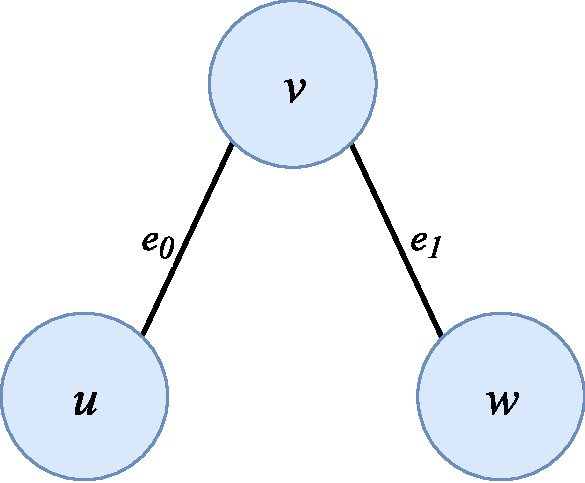
\includegraphics[scale=0.4]{grafo-simples}
\centering
\caption{Representação gráfica de G$_{1}$.}
\end{figure}

%%%%%
\subsection{Grafo Completo}
\label{conceitos__grafo--comleto}

Um \emph{grafo completo} G é um grafo onde cada par de vértices é conectado por uma aresta, ou seja, $|E[G]| = \frac{n(n-1)}{2}$, que é o número máximo de arestas que um grafo pode ter, onde \emph{n} = |V[G]|.

\begin{figure}[H]
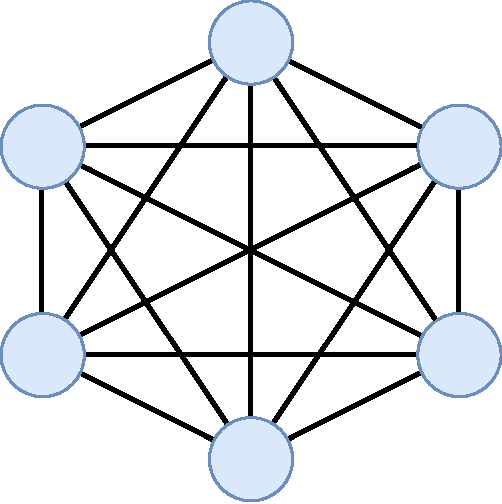
\includegraphics[scale=0.5]{grafo-completo}
\centering
\caption{Representação gráfica de um grafo completo com seis vértices.}
\end{figure}

%%%%%
\subsection{Densidade}
\label{conceitos__grafo--densidade}

A \emph{densidade} de um grafo G é a razão entre a quantidade de arestas G e a quantidade de arestas em um grafo completo com o mesmo número de vértices. Caso a densidade de G seja alta, é dito que G é um grafo \emph{denso} e, caso contrário, ele é considerado um grafo \emph{esparso}.

%%%%%
\subsection{Clique}
\label{conceitos__grafo--clique}

Uma \emph{clique} C em um grafo G é um subconjunto de vértices tais que cada par de vértices do subconjunto é conectado por uma aresta. Isso significa dizer C que é um \emph{subgrafo} de G, $C \subseteq G$, e que C é completo, ou seja, $|E[C]| = \frac{n_{c}(n_{c}-1)}{2}$, onde $n_{c}$ = |V[C]|.

% \begin{figure}[H]
% 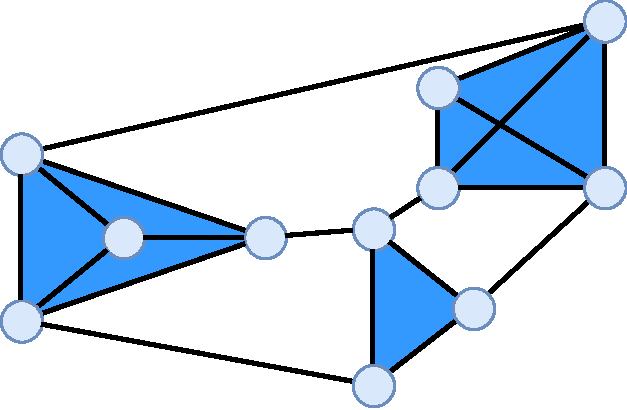
\includegraphics[scale=0.4]{grafo-clique}
% \centering
% \caption{Representação gráfica de um grafo com cliques, onde cada área colorida representa uma clique}
% \end{figure}

%%%%%
\subsection{Peso}
\label{conceitos__grafo--peso}

Grafos são muito utilizados para modelar problemas reais e, em certos problemas, é preciso incluir alguns atributos especiais, como por exemplo um custo, que está associado com as arestas. Em uma rede de tráfego, por exemplo, esse custo poderia representar a distância entre dois lugares. Esses problemas costumam ser modelados por um grafo ponderado.

Para cada aresta \emph{e} de um grafo G, é associado um número real \emph{w}(\emph{e}), denominado \emph{peso}. Sendo assim, G, com o atributo peso associado as arestas, é chamado de \emph{grafo ponderado}.

%%%%%
\subsection{Grau de um vértice}
\label{conceitos__grafo--grau}

\def \variable {\emph{v}}

O \emph{grau} de um vértice \emph{v} em um grafo G, denotado por \emph{d$_{G}$}(\emph{v}), é o número de arestas em G que incidem sobre \emph{v}. De modo particular, \emph{d$_{G}$}(\emph{v}) é o número de vizinhos de \emph{v} em G. Um vértice de grau zero é chamado de \emph{vértice isolado}. O grau mínimo e o grau máximo dos vértices de G são denotados por $\delta(G)$ e $\Delta(G)$, respectivamente, enquanto que \emph{d}(G) denota seu \emph{grau médio}, $\frac{1}{n}\sum_{v\in V}(d(v))$, onde \emph{n} é o número de vértices de G~\cite{bondy1976graph}.

Em um grafo ponderado, o grau de um vértice \emph{v} é dado pela soma dos pesos das arestas que incidem sobre \emph{v}.

%%%%%
\subsection{Componente}
\label{conceitos__grafo--componente}

Um grafo é dito \emph{conexo} se, para cada par de vértices, existe um \emph{caminho} entre eles, ou seja, uma sequência de vértices onde cada par consecutivo na sequência é ligado por uma aresta.

Quando um grafo não é conexo, ele se divide em \emph{componentes}, que são subconjuntos de vértices desse grafo, onde cada par destes vértices possui um caminho entre eles, ou seja, a componente é conexa. Além disso, as componentes são isoladas, ou seja, não existe aresta ligando vértices de diferentes componentes.

\begin{figure}[H]
    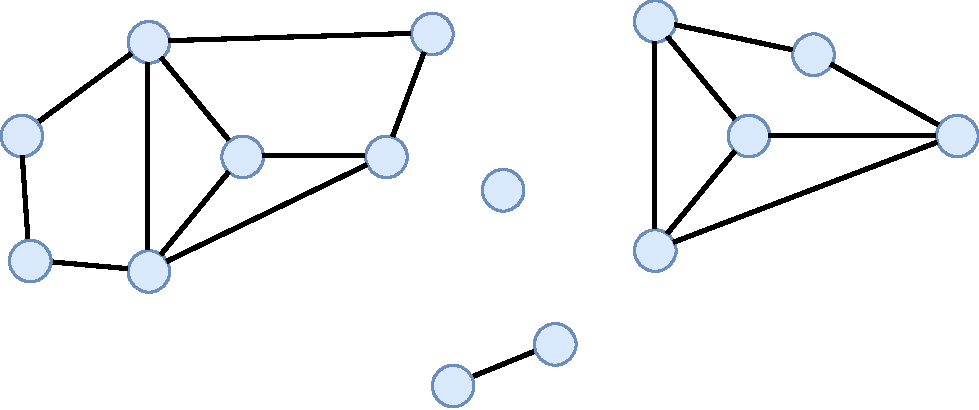
\includegraphics[scale=0.4]{grafo-componentes}
    \centering
    \caption{Grafo dividido em quatro componentes. Nota-se que um vértice isolado também pode ser visto como uma componente.}
\end{figure}

%%%%%
\subsection{Componente Gigante}
\label{conceitos__grafo--componente-gigante}

\emph{Componente gigante}~\cite{easley2010networks} é um termo informal utilizado para
um componente conexo que contém uma fração significativa de todos os vértices de um grafo. Além disso, quando um grafo contém um componente gigante, quase sempre este componente é único.

Na figura \ref{fig:grafo-componente-gigante}, é apresentado uma rede de relacionamentos românticos em uma escola secundária americana. É possível identificar uma componente gigante, onde até estudantes com apenas uma relação estão incluídos nela. Também é fácil perceber que, basta que uma pessoa de uma das componentes menores ter um relacionamento com alguém da componente gigante, que todos os vértices desta componente passarão a fazer parte da componente gigante.

É por este motivo que, quase sempre, uma componente gigante é única em uma rede, pois basta uma aresta de uma componente a outra para que elas se unam, formando uma nova componente única.

\begin{figure}[H]
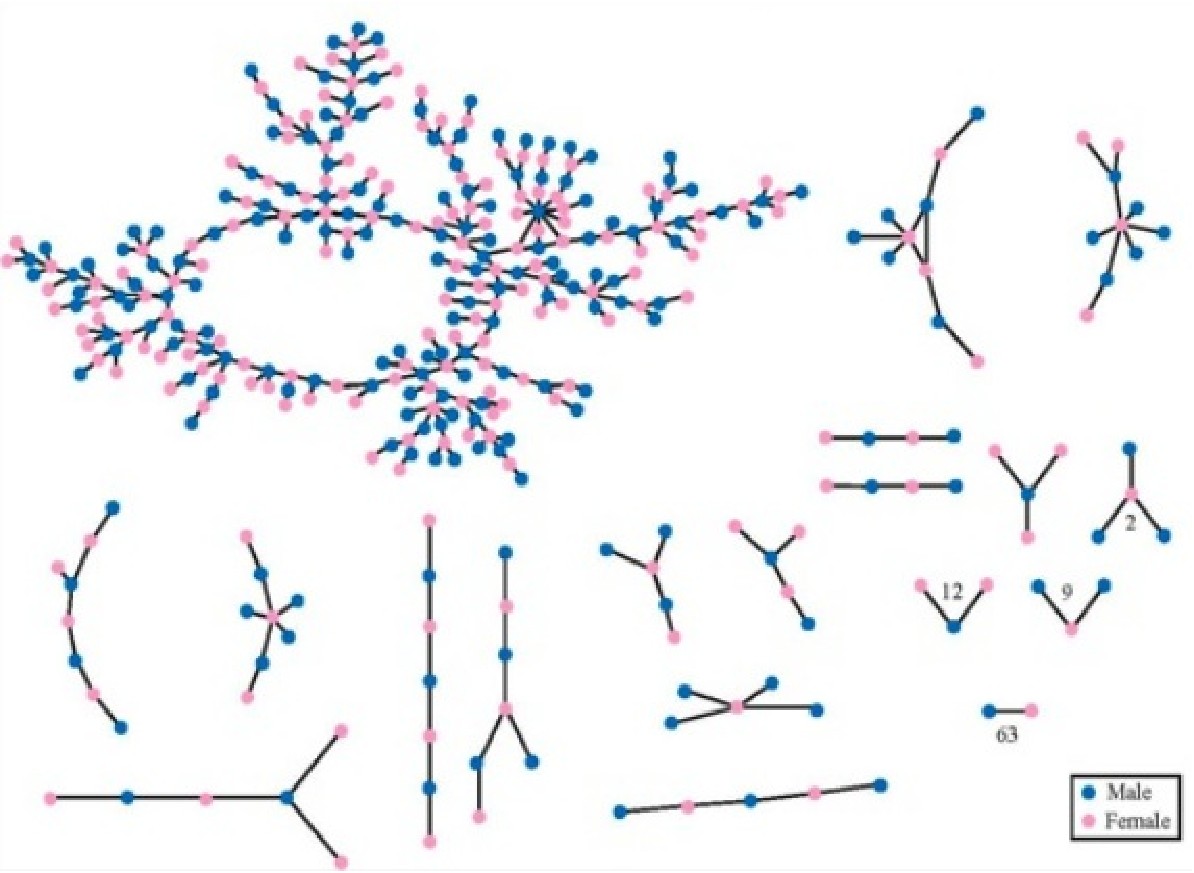
\includegraphics[scale=0.6]{grafo-componente-gigante}
\centering
\caption{
    Rede de relacionamentos românticos em uma escola secundária americana num período de 18 meses. Fonte:~\cite{bearman2004chains}.
}
\label{fig:grafo-componente-gigante}
\end{figure}

%%%%%%%%%%%%%%%%%%%%%%%%%%%%%%%%%%%%%%%%%%%%%%%%%%%%%%%%%%%
% \subsection{Fechamento Triádico}
% \label{conceitos__grafo--fechamento-triadico}

% Na maioria dos estudos de redes sociais, é interessante entender como uma rede evolui através do tempo. O \emph{fechamento triádico} é um princípio básico que auxilia esse entendimento, através da formação de novas arestas.

% Claro que as alterações que as arestas de uma rede podem sofrer dependem muito
% do tipo de rede que está sendo analisada, porém, o princípio do fechamento tríadico é definido basicamente da seguinte maneira:


% \begin{quotation}
%     \emph{Se duas pessoas em uma rede social têm um amigo em comum, então há
% uma probabilidade maior de se tornarem amigos em algum momento do fu-
% turo}~\cite{rapoport1953spread}.
% \end{quotation}

% A figura \ref{fig:grafo-fechamento-triadico} ilustra exemplos de fechamentos triádicos. Os vértices \emph{A} e \emph{E} tem o vértice \emph{B} em comum, então a formação de uma nova aresta \emph{A}-\emph{E} produz uma situação onde os três vértices estão conectados. Essa estrutura de três vértices é chamada de \emph{triângulo}. O termo \emph{fechamento triádico} vem do fato de que a aresta \emph{A}-\emph{E} teve o efeito de ‘‘fechar’’ o terceiro lado deste triângulo. Neste exemplo, o mesmo comportamento ocorre com as arestas \emph{B}-\emph{F} e \emph{D}-\emph{G}.
%
% Ao observar grandes redes sociais por um período de tempo, é comum identificar esse tipo de comportamento de fechamento triádico.
%
% \begin{figure}[H]
%     \center
%     \subfigure[fig:fechamento-triadico-antes][Antes de formar novas arestas]{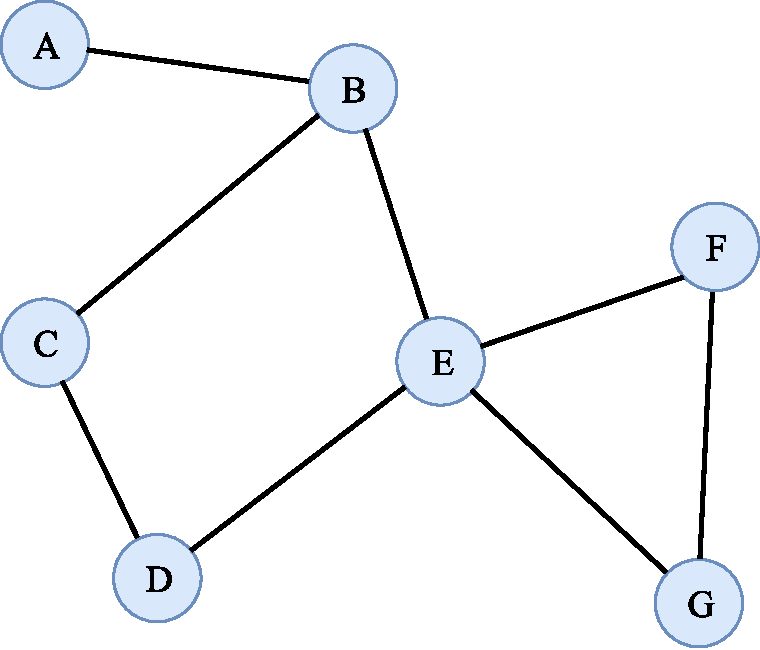
\includegraphics[width=6cm]{fechamento-triadico-antes}}
%     \qquad
%     \subfigure[fig:fechamento-triadico-depois][depois de formar novas arestas]{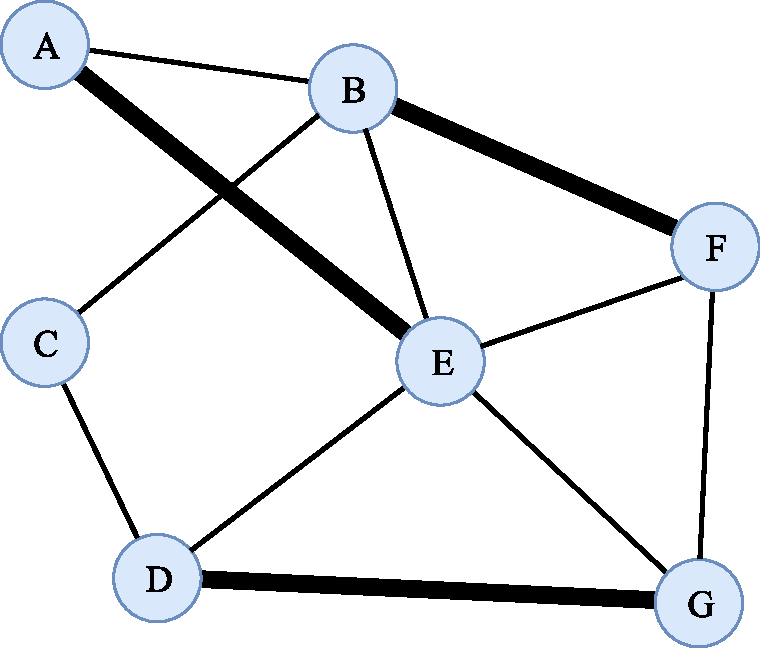
\includegraphics[width=6cm]{fechamento-triadico-depois}}
%
%     \caption{Ao observar uma rede por um período de tempo, é possível ver que novas arestas são formadas, muitas vezes seguindo o princípio do fechamento triádico.}
%     \label{fig:grafo-fechamento-triadico}
% \end{figure}
%
% %%%%%
% \subsection{Coeficiente de clustering}
% \label{conceitos__fechamento-triadico--coeficiente-clustering}
%
% A regra do fechamento triádico motiva a definição de algumas métricas. Uma delas é o coeficiente de \emph{clustering}.
%
% O \emph{coeficiente de clustering} de um vértice \emph{v} é a probabilidade de que dois de seus vizinhos, selecionados aleatoriamente, sejam conectados por uma aresta.
%
% Na figura \ref{fig:grafo-fechamento-triadico}, por exemplo, o vértice \emph{E} possui coeficiente de \emph{clustering} $\frac{1}{6}$ antes da formação de novas arestas, pois, como \emph{E} tem quatro vizinhos, o número máximo de arestas que poderiam ser formadas entre eles é seis, mas só existe uma. Após a formação de novas arestas, \emph{E} passa a ter um coeficiente de \emph{clustering} de $\frac{4}{10}$.
%
% O \emph{coeficiente de clustering médio} de um grafo é dado por $\bar{C = \frac{1}{n}\sum_{v\in V}(C_{v})$, onde $C_{v}$ é o coeficiente de \emph{clustering} do vértice \emph{v}.
%
% \todo{Será que precisa colocar algo sobre coeficiente de clustering em grafo ponderado? Pq e é diferente e como os nossos grafos são ponderados... Mas não tem mto material por aí}
%
% \todo{ver depois:}
%
% \url{https://arxiv.org/pdf/cond-mat/0311416.pdf}
%
% \url{https://toreopsahl.com/tnet/weighted-networks/clustering/}
%
% \url{http://citeseerx.ist.psu.edu/viewdoc/download?doi=10.1.1.139.9018&rep=rep1&type=pdf}

%%%%%%%%%%%%%%%%%%%%%%%%%%%%%%%%%%%%%%%%%%%%%%%%%%%%%%%%%%%
\section{\texorpdfstring{\MakeUppercase{Homofilia}}{}}
\label{conceitos__homofilia}

Um dos princípios mais básicos em redes sociais é o de \emph{Homofilia}. Este princípio diz que as pessoas tendem a ser semelhantes aos seus amigos. Ao observar grupos de amigos, é comum ver que as pessoas de cada grupo compartilham várias características, como por exemplo etnia, idade, interesses, crenças, etc. Claro que as redes sociais não se limitam a este comportamento somente, podendo existir conexões entre pessoas com características diferentes, mas de maneira generalizada, as conexões são formadas entre semelhantes~\cite{easley2010networks}.

\begin{figure}[H]
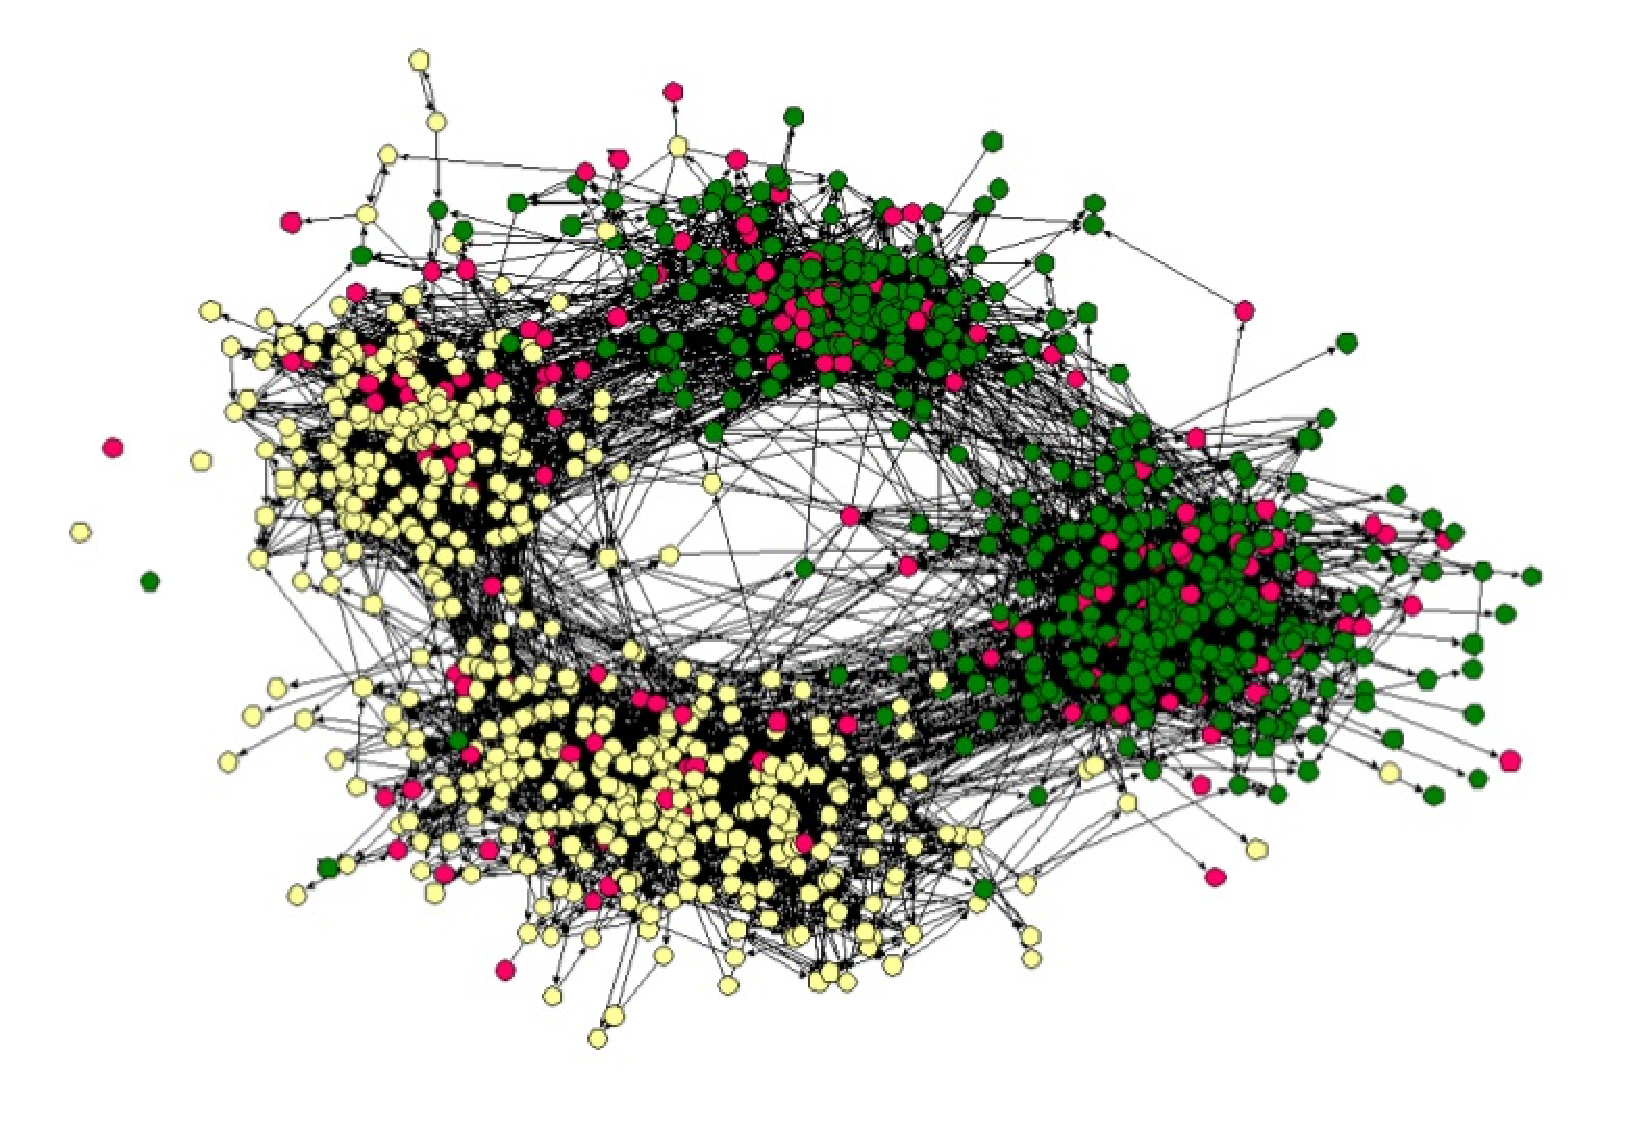
\includegraphics[scale=0.6]{grafo-homofilia}
\centering
\caption{
     Exemplo de homofilia em uma rede social, onde é possível visualizar duas divisões na rede. A primeira - da esquerda para a direita - leva em consideração a raça dos indivíduos, representada pela coloração dos vértices, e a segunda - de cima para baixo - é baseada na idade escolar. Fonte:~\cite{moody2001race}.
}
\label{fig:grafo-homofilia}
\end{figure}

%%%%%%%%%%%%%%%%%%%%%%%%%%%%%%%%%%%%%%%%%%%%%%%%%%%%%%%%%%%
\section{\texorpdfstring{\MakeUppercase{Modularidade e Comunidades}}{}}
\label{conceitos__modularidade}

Muitos dos problemas representados por uma estrutura de grafos apresentam \emph{comunidades} (ou \emph{clusters}), que podem ser definidas como subconjuntos de vértices que podem ser facilmente agrupados, pois são densamente conectados internamente, porém esparsamente conectados com o restante do grafo. Assim, é interessante identificar estas comunidades para analisá-las separadamente, pois podem ter diferentes propriedades, tais como grau dos vértices, coeficiente de \emph{clustering}, centralidade, etc.

\emph{Modularidade} é a medida que busca a divisão de um grafo em comunidades. Quanto maior a modularidade de um grafo, maior a densidade nas conexões entre vértices de uma mesma comunidade.

%%%%%%%%%%%%%%%%%%%%%%%%%%%%%%%%%%%%%%%%%%%%%%%%%%%%%%%%%%%
\section{\texorpdfstring{\MakeUppercase{Sistema Eleitoral Brasileiro}}{}}

A Constituição Federal, através do Código Eleitoral, define o sistema eleitoral brasileiro como um sistema misto, com eleições \emph{majoritárias} para os cargos executivos, - Prefeitura, Senado e Presidência - e \emph{proporcionais} para os cargos legislativos - Câmara dos Deputados, Assembleias Legislativas e Câmaras Municipais - onde podem concorrer às eleições somente candidatos registrados por partidos políticos.~\cite{brasil1965lei4737}. Além disso, o sistema eleitoral brasileiro é regulado pelo \gls{TSE}.

%%%%%%%%%%%%%%%%%%%%%%%%%%%%%%%%%%%%%%%%%%%%%%%%%%%%%%%%%%%
\section{\texorpdfstring{\MakeUppercase{Partidos Políticos no Brasil}}{}}
\label{conceitos__partidos-brasil}

Segundo a  Lei nº 9.096, de 1995, que dispõe sobre partidos políticos, o \emph{partido político}, no interesse do regime democrático, destina-se a assegurar a autenticidade do sistema representativo e a defender os direitos fundamentais definidos na Constituição Federal~\cite{brasil1995lei9096}. Ou, segundo Vera Maria Nunes Michels:

\begin{quotation}
    \emph{Podemos entender, assim, que o partido político, como pessoa jurídica de direito privado, é um grupo social de relevante amplitude, destinado à arregimentação coletiva, em torno de ideias e de interesses, para levar seus membros a compartilhar do poder decisório nas instâncias governamentais}~\cite{michels2006direito}.
\end{quotation}

De modo geral, é possível definir um partido político como um grupo de pessoas com ideias em comum sobre pautas políticas e sociais com o objetivo de formar planos governamentais de acordo com estas ideias~\cite{garibaldi2017partidos}.

Por questões de praticidade, neste trabalho, os partidos políticos serão denotados apenas por \emph{partidos}.

%%%%%%%%%%%%%%%%%%%%%%%%%%%%%%%%%%%%%%%%%%%%%%%%%%%%%%%%%%%

\section{\texorpdfstring{\MakeUppercase{Coligações Partidárias}}{}}
\label{conceitos__coligacoes}

É comum que diferentes partidos políticos compartilhem ideias, ideais e/ou interesses, de modo que formam alianças entre si. Estas alianças são permitidas e regulamentadas na maioria das democracias e no Brasil não é diferente, sendo então chamadas de \emph{Coligações Partidárias} ou simplesmente \emph{Coligações}.

No Brasil, as Coligações são formadas, de maneira formal, durante o período de campanha eleitoral e seguem algumas regras~\cite{brasil1997lei9504}, sendo as mais importantes, para o contexto deste trabalho, as listadas abaixo:

\begin{itemize}
    \item Um partido pode fazer parte de coligações somente em eleições majoritárias, somente em eleições proporcionais ou em ambas; e
    \item Caso o partido esteja em coligações em ambas as eleições - majoritárias e proporcionais - este partido partido não pode fazer coligação, em eleições proporcionais, com partidos pertencentes a coligações concorrentes nas eleições majoritárias. Sendo esta regra válida por região eleitoral (municipal, estadual ou nacional).
\end{itemize}

Um exemplo básico que ocorre frequentemente nas eleições brasileiras, é o caso de dois partidos que podem estar na mesma coligação para a disputa presidencial, estarem em coligações diferentes para uma disputa para governador em um estado específico, mas em outro estado, estarem na mesma coligação.

Neste trabalho, é dito que ‘‘um partido faz coligação com outro’’ como forma de dizer que dois partidos pertencem a uma mesma coligação.

%%%%%%%%%%%%%%%%%%%%%%%%%%%%%%%%%%%%%%%%%%%%%%%%%%%%%%%%%%%

\section{\texorpdfstring{\MakeUppercase{Espectro Político}}{}}
\label{conceitos__espectro-politico}

Nas seções anteriores, vimos que partidos e coligações se reúnem, em teoria, através de ideais em comum. Um sistema utilizado para classificar ideologias e posições políticas é o \emph{espectro político}.

No modelo mais básico de espectro político, que será utilizado neste trabalho, as posições políticas costumam ser rotuladas como de \emph{extrema esquerda}, \emph{esquerda}, \emph{centro-esquerda}, \emph{centro}, \emph{centro-direita}, \emph{direita} e \emph{extrema direita} e colocadas ao longo de um eixo. Este modelo surge no parlamento francês no século XVIII onde, para fazer a distinção de ideais políticos, os parlamentares sentavam-se à esquerda ou à direita no plenário, conforme o seu alinhamento com certas correntes políticas.

\begin{figure}[H]
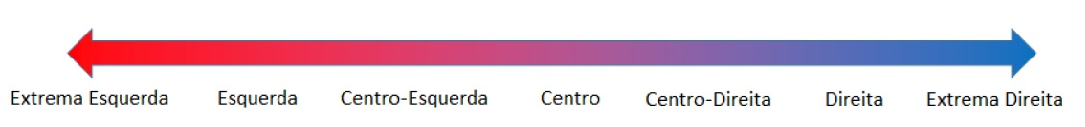
\includegraphics[width=1\textwidth]{eixo-esquerda-direita}
\centering
\caption{
    Representação do espectro político Esquerda-Direita sobre um eixo. Fonte:~\cite{matos2016esquerdadireita}.
}
\label{fig:eixo-esquerda-direita}
\end{figure}

\todo{precisa falar aqui que a gente não precisa entrar em detalhes que explicam exatamente o que é direita x esquerda, ou precisa falar sobre mais especificamente?}

%%%%%%%%%%%%%%%%%%%%%%%%%%%%%%%%%%%%%%%%%%%%%%%%%%%%%%%%%%%

\section{\texorpdfstring{\MakeUppercase{Visualizações}}{}}
\label{conceitos__visualizacoes}

Para a representação gráfica dos grafos foi utilizada a plataforma \emph{Gephi}\footnote{\url{https://gephi.org/}}, um software com licença de código aberto amplamente utilizado para esta finalidade, onde basta importar um arquivo em formato específico para gerar uma visualização do grafo correspondente. Além disso, o \emph{Gephi} fornece vários \emph{plugins} que podem ser utilizados para executar algoritmos sobre o grafo desejado. Estes \emph{plugins} foram utilizados para calcular várias das métricas apresentadas neste trabalho, como \emph{modularidade}, \emph{grau médio} e \emph{densidade}, facilitando consideravelmente a análise.

O \emph{Gephi} também disponibiliza várias formas de visualização de um grafo e dentre estas foram utilizadas duas, \emph{Force Atlas 2} e \emph{Fruchterman-Reingold}, as quais serão explicadas superficialmente, pois no contexto deste trabalho não convém entrar em detalhes de implementação.

As figuras \ref{fig:grafo-force-atlas} e \ref{fig:grafo-fruchterman-reingold} mostram estas visualizações a partir de um grafo que representa colaborações entre músicos de jazz, onde cada músico é representado por um vértice e, se dois músicos fizeram parte de uma mesma banda, não necessariamente ao mesmo tempo, uma aresta se forma sobre os vértices que os representam~\cite{gleiser2003list}.

\subsection{Force Atlas 2}
\label{conceitos__visualizacoes--force-atlas}

O algoritmo de visualização Force Atlas 2~\cite{jacomy2014forceatlas2} é baseado em força, onde os vértices se repulsam, como se fossem partículas carregadas, e então as arestas atraem os vértices sobre os quais incidem, como as molas. Esta visualização também leva em consideração o peso das arestas e é muito útil quando espera-se uma divisão em comunidades no grafo a ser analisado, pois vértices pertencentes a uma mesma comunidade tendem a ficar próximos.

\begin{figure}[h]
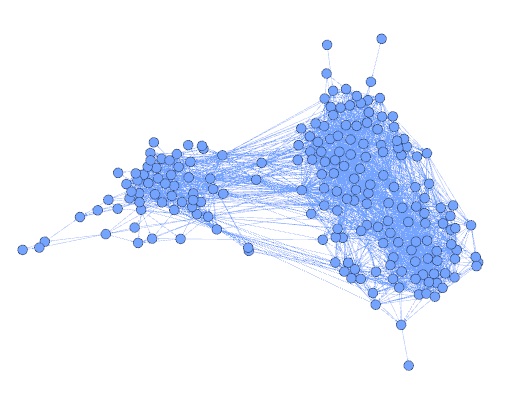
\includegraphics[scale=0.6]{grafo-force-atlas}
\centering
\caption{
    Grafo visualizado utilizando Force Atlas 2.
}
\label{fig:grafo-force-atlas}
\end{figure}

%%%%%
\subsection{Fruchterman-Reingold}
\label{conceitos__visualizacoes--fruchterman-reingold}

O Algoritmo de visualização \emph{Fruchterman-Reingold}~\cite{fruchterman1991graph} também é baseado em força, porém sem levar em consideração o peso das arestas. Esta visualização segue dois princípios básicos:

\begin{enumerate}
\item Vértices conectados por uma aresta devem ficar próximos;
\item Vértices não devem ficar \emph{próximos demais} uns dos outros.
\end{enumerate}

Sendo assim, o algoritmo distribui os vértices uniformemente, tornando também o tamanho das arestas uniforme e refletindo simetria.

\begin{figure}[h]
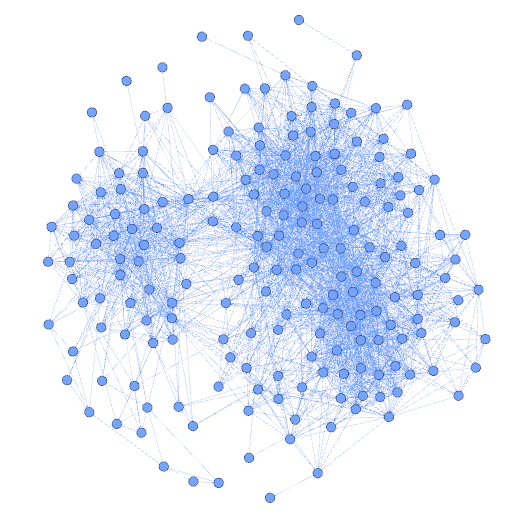
\includegraphics[scale=0.6]{grafo-fruchterman-reingold}
\centering
\caption{
    Mesmo grafo da figura \ref{fig:grafo-force-atlas}, porém utilizando a visualização Fruchterman-Reingold.
}
\label{fig:grafo-fruchterman-reingold}
\end{figure}
